%In \cite{li2015subisit,li2015subdraft}, two schemes have been proposed to recover the support of a $K$-sparse $N$-dimensional signal from noisy linear measurements. Both schemes use left-regular sparse-graph code based sensing matrices and a simple peeling-based decoding algorithm. Both the schemes require $O(K \log N)$ measurements and the first scheme require $O(N \log N)$ computations whereas the second scheme requires $O(K \log N)$ computations (sub-linear time complexity when $K$ is sub-linear in $N)$. We show that by replacing the left-regular ensemble with left and right regular ensemble, we can reduce the number of measurements required of these schemes to the optimal order of $O\left(K \log \frac{N}{K} \right)$ with decoding complexities of $O(K \log \frac{N}{K})$ and $O(N \log \frac{N}{K})$, respectively.

\section{Introduction}
The classical problem of compressed sensing involves estimating a signal $\mbf{x}$, which is sparse in some basis, from a noisy measurement signal $\mbf{y}$ of smaller dimension compared to $\mbf{x}$. Formally, let
\begin{align*}
\mbf{y=Ax+w},
\end{align*}
where $\mbf{x}$ is an $N$-dimensional vector, $\mbf{A}$ is a known $M \times N$ matrix commonly referred to as \emph{measurement matrix} and $\mbf{w}$ is additive noise. The unknown signal $\mbf{x}$ is known to be sparse in some basis and we denote the sparsity of $\mbf{x}$ by $K$. If there is no noise, then we refer to it as the noiseless setting. It is known that if $K \ll N$ we can recover the unknown signal in significantly fewer number of measurements compared to $N$.  Particularly in this chapter we focus on recovering the support of $\mbf{x}$ defined as supp$(\mbf{x}):=\{i:x_i\neq 0, i\in[N]\}$ where $\mbf{x}=[x_1,\ldots , x_i \ldots ,x_N]^{T}$ and $[N]\coleq\{1,2,\ldots ,N\}$. For a given scheme, given the reconstruction vector $\widehat{\mbf{x}}$, we consider the probability of failure of support recovery which can be defined as
\begin{align*}
\mbb{P}_{F}\coleq\Pr(\text{supp}(\widehat{\mbf{x}})\neq \text{supp}(\mbf{x})).
\end{align*}
 For the support recovery problem, under noisy settings, Wainwright \cite{wainwright2009information} showed information theoretically that $O\left(K\log(\frac{N}{K})\right)$ number of measurements is necessary and sufficient for asymptotically reliable recovery.

In \cite{li2015subisit} (and in the expanded version in \cite{li2015subdraft}), Li, Pawar and Ramchandran have considered the compressed sensing problem of recovering the support of a $K$-sparse, $N$-dimensional signal from $M$ linear and noisy measurements. Based on sparse-graph codes with a \emph{left-regular} degree profile and a peeling decoder, they have proposed an elegant design of the measurement matrix and a recovery algorithm. They have proposed two designs - the first design requires $M = \mc{O}(K \log N)$ measurements and a near-linear $\mc{O}(N \log N)$ decoding complexity, whereas the second design requires $M = \mc{O}(K \log N)$ measurements with a sub-linear $\mc{O}(K \log N)$ decoding complexity.
%This combination is shown to provide order-wise optimal measurement complexity (number of measurements) and computational complexity.

In this chapter\cite{vem2016sub}, we show that the bounds on the measurement complexity reported in \cite{li2015subisit,li2015subdraft} can be improved by considering \emph{left-and- right-regular} sparse-graph based sensing matrices. We show that only $\mc{O}\left(K \log \frac{N}{K} \right)$ measurements are required when $K = \mc{O}(N^\delta)$, for any $0 \leq \delta < 1$, to recover the support with the optimal sub-linear time decoding complexity.  This matches the information-theoretic lower bound on the number of measurement required for asymptotically-reliable recovery \cite{wainwright2009information}. Also, through simulations we demonstrate that the proposed scheme has superior performance compared to \cite{li2015subdraft}.
%For sub-linear time decoding complexity, we show that only $O\left(K \log^{1.3} \frac{N}{K} \right)$ are required. Finally, we also provide sharper version of the results in \cite{li2015subdraft}. 

The literature on compressed sensing is vast and it is difficult to provide a comparison with several of the existing results in the literature due to different error performance metrics being used for different versions of the problem. Nevertheless, it should be pointed out that the use of left and right regular bipartite graphs as choice for sensing matrix has been proposed in \cite{jafarpour2009efficient} and the measurement complexity has been shown to be only $\mc{O}\left(K \log \frac{N}{K} \right)$. However, the decoding complexity is near-linear $\mc{O}(N\log \frac{N}{K})$. We achieve a similar measurement complexity but with optimal computational complexity of $\mc{O}(K\log \frac{N}{K})$. Also unlike in \cite{jafarpour2009efficient} the sensing matrix in this chapter is constructed based on a tensor-product construction and the decoding algorithm is based on identifying singletons and peeling them off.

% sensing scheme and the decoding algorithm in this chapter are different from those in \cite{jafarpour2009efficient} and are based directly on those in \cite{li2015subisit,li2015subdraft}. 
 
For the information-theoretic lower bound in \cite{wainwright2009information} to hold, the non-zero elements in $\mbf{x}$ should have a sufficiently large minimum absolute value. In view of this condition, similar to \cite{li2015subisit,li2015subdraft}, we assume that all the non-zero elements of $\mbf{x}$ belong to the set $\{Ae^{i\theta}:A\in\mc{A},\theta\in\Theta\}$ where $\mc{A}\coleq \{A_{\text{min}}+\rho l\}^{L_1}_{l=0},\Theta\coleq\{2\pi l/L_2\}_{l=0}^{L_2}$ for finite but arbitrarily large integers $L_1$ and $L_2$.

%we set a minimum absolute value for the non-zero elements and further assume that they are from a discrete set. More precisely for the noisy setting
\section{Prior work}
\label{Sec:Review}
In this section, we review the construction of the measurement matrix $\mbf{A}$ proposed by Li, Pawar and Ramchandran in \cite{li2015subisit} and \cite{li2015subdraft}, and also summarize their key results. To keep the discussion simple, we omit certain details and refer readers to the original work \cite{li2015subisit} (and the expanded version  \cite{li2015subdraft}).

%The main idea is to use the sparse-graph based construction to decompose the problem of $K$-sparse support recovery into 1-sparse problems and then use a simple peeling based decoder \cite{richardson2008modern} to recover the support.
The measurement matrix is constructed using a combination of a sparse-graph code defined by the $R \times N$ coding matrix ${\bf H=[h_1, h_2, \cdots ,h_{N}]} \in {\{0,1 \}}^{R \times N}$  and a $P \times N$ bin-detection matrix $\bf S=[s_1, s_2, \cdots ,s_N]$. The coding matrix $\bf H$ defines a bipartite graph $\mathcal{G}$ with $N$ left (variable) nodes, representing the $N$-length signal $\bf x$, and $R$ right (check) nodes representing the measurements  $\bf y=[y_1, y_2, \cdots, y_R]$. Let $q_i, i\in [R]$, be the number of non-zero variable nodes connected to $i^{\text{th}}$ check node. Assume an ``oracle" that solves the 1-sparse problem by examining each check node observations and classifies it as a zero-ton($q_i=0$), singleton($q_i=1$) or a multi-ton($q_i>1$), and also identifies the position $\hat{k}$ and value $\widehat{x}_{\hat{k}}$ of the participating variable node if it is a single-ton. Once a singleton is identified the corresponding variable node's contribution is peeled off from other participating check nodes and this process creates new single-tons. The decoding process continues until there are no more singletons. The decoding is successful if all the $K$ non-zero elements of $\bf x$ are recovered at the end of decoding.

The  $RP \times N $ measurement matrix $\bf A$ with $M = RP$ measurements is constructed by taking the row tensor product $ \boxtimes$ of $\bf H$ and $\bf S$ given by
\[
 \bf A = H \ { \boxtimes} \ S := [h_1 \otimes s_1, h_2 { \otimes} s_2, \cdots , h_N { \otimes} s_N]
 \]

where $\otimes$ is the standard Kronecker product.

%They explore both $\textit{l}$-left regular and irregular ensembles for the $\bf H$ matrix construction and provide analysis for the left regular case.
For the noisy setting, they have proposed three designs for $\bf S$ which essentially performs the role of the oracle in identifying a single-ton at each check node. These designs are \emph{RandomNoisy} with near-linear decoding complexity, \emph{BinaryNoisy} and \emph{FourierNoisy} each with sub-linear decoding complexity.
%The only difference in these designs is the $\bf S$ matrix construction and hence the 1-sparse(bin detection) problem solving methodology.
The bin-detection matrix $\bf S$ for the three settings are as follows:
\begin{itemize}
\item \emph{RandomNoisy:}  Ensemble of $P \times N$ matrices $S = [S_{i,j}]_{P \times N}$ where $S_{i,j}$ $’$s are i.i.d. sub-gaussian entries with zero mean and unit variance.

\item  \emph{FourierNoisy}:  $\bf S = [S_0 S_1 \cdots S_{P-1}]^{T}$, where $\bf S_p$ consists of $Q=O(\log^{1/3}N)$ consecutive $2^p$-dyadically spaced rows from the $N \times N$ DFT matrix.

\item \emph{BinaryNoisy:}  $\mbf{S} = f(\mbf{C})$ where $\mbf{C}_{P \times N}$ is a binary codebook(or subset of a codebook) of a linear code with block length $P$, $f:\{0,1\}^q\rightarrow \mc{M}$ is a modulation scheme that maps $C_{P \times N}$ to $S_{\frac{P}{q}\times N}$. For e.g., for QAM $q=2$ and $\mc{M}=\{\pm 1 \pm i\}$.
\end{itemize}

The following theorems from \cite{li2015subdraft} summarize their key results.

%\begin{theorem}[\cite{li2015subdraft} Noiseless recovery]\label{thm:li1}
%In the absence of noise, given any $K$-sparse signal $\mbf{x}$ with $x_k \in \mathcal{X}$ for $k \in \text{supp} \mbf{(x)}$, their noiseless recovery schemes achieve a vanishing failure probability $\mathbb{P}_F(O\left(\frac{1}{K})\right) \rightarrow 0$ asymptotically in $K$ and $N$ with
%\begin{center}\small
%\begin{tabular}{|c|c|c|}
%  \hline
%   &  $M$ &  $T$ \\
%  \hline
%  Fourier noiseless & $2(1+\epsilon)K$ & $O(K)$ \\
%  \hline
%  Binary noiseless & $(1+\epsilon)K(\log_2 N+1)$ & $O(K \log N)$ \\
%  \hline
%\end{tabular}
%\end{center}
%where $M$ and $T$ are measurement cost and computational complexity respectively.
%\end{theorem}
%\vspace{2ex}


\begin{theorem}[\cite{li2015subdraft} Sub-linear Time Noisy Recovery]\label{thm:li2} In the presence of i.i.d. Gaussian noise with zero mean and
variance $\sigma^2$, given any $K$-sparse signal $\mbf{x}$ with $x_k \in \mathcal{X}$ for $k \in \text{supp}(\mbf{x})$, our noiseless recovery schemes achieve a vanishing failure probability $\mathbb{P}_F \rightarrow 0$ asymptotically in $K$ and $N$ with
\begin{center}\small
\begin{tabular}{|c|c|c|}
  \hline
   & $M$ &  $T$ \\
  \hline
  Fourier noisy & $O(K \log^{1.3}N)$ & $O(K \log^{1.3}N)$ \\
  \hline
  Binary noisy & $O(K \log N)$ & $O(K \log N)$ \\
  \hline
\end{tabular}
\end{center}
where $M$ and $T$ are measurement cost and computational complexity respectively.
\end{theorem}
\vspace{2ex}

\begin{theorem}[\cite{li2015subdraft} Near-linear Time Noisy Recovery]\label{thm:li3} In the presence of i.i.d. Gaussian noise with zero mean and
variance $\sigma^2$, given any $K$-sparse signal $\mbf{x}$ with $x_k \in \mathcal{X}$ for $k \in \text{supp}(\mbf{x})$, the RandomNoisy scheme achieves a vanishing failure probability $\mathbb{P}_F \rightarrow 0$ asymptotically in $K$ and $N$ with a measurement complexity of $M = O(K \log N)$ and computational complexity of $T = O(N \log N)$.
\end{theorem}

\section{Proposed scheme}
%\subsection{Main Idea}
The main difference between \cite{li2015subdraft} and our approach is that we replace the left $l$-regular ensemble of graphs corresponding to the coding matrix $\mbf{H}$ described in Sec \ref{Sec:Review} by left {\em and} right $\left(l, r\right)$-regular ensemble of graphs.

\begin{definition}[Left and right regular graph ensemble]\label{def:leftandrighreg}
Let $\mathcal{G}^N_{\rm reg,reg}\left(R,l, \frac{lN}{R} \right)$ denote the ensemble of left and right regular bipartite graphs with $N$ variable nodes and $R$ check nodes, where each variable node $k \in [N]$ is connected to $l$ check nodes and each check node $j \in [R]$ is connected to $\frac{lN}{R}$ left nodes.
\end{definition}
In the design considerations of bin detection matrix, we now have only $r=\frac{lN}{\eta K}=O\left(\frac{N}{K}\right)$ variable nodes connected to each check node and thus we require only a bin detection matrix $\mbf{S}$ with $O(\frac{N}{K})$ columns. For the bin detection matrix designs in Sec. \ref{Sec:Review} we know from \cite{li2015subdraft} that to differentiate between a zero-ton, singleton and a multi-ton successfully with probability approaching $1$ asymptotically in $\frac{N}{K}$ we only require $\log(\frac{N}{K})$ rows in $\mbf{S}$. We choose the bin detection matrix to be similar to the \emph{RandomNoisy, FourierNoisy, BinaryNoisy} designs but with dimensions $P'\times r$ where $P'=O\left(\log(\frac{N}{K})\right)$.

We know from the modern coding theory that to peel off $K$ unknown variable nodes successfully from the bipartite graph we need $\eta K$ number of check nodes for some $\eta>1$. So we choose the number of check nodes $R = \eta K$. A matrix $\mathbf{H}$ is chosen at random from this ensemble $\mathcal{G}^N_{\rm reg,reg}\left(\eta K,l, \frac{lN}{\eta K} \right)$ and used as the coding matrix.

The measurement matrix $\bf A$ for the proposed construction with $\bf H_{R \times N} = [h_1, h_2, \cdots, h_N]^{T}$ and $\bf S_{P' \times r}= [s_1, s_2, \cdots ,s_r]$ is given by $ {\bf A}_{RP' \times N} = {\bf H \boxplus S }$,
 where $ \boxplus$ is the new tensoring operation, which is slightly different from the row-tensor operation used in Sec \ref{Sec:Review} and is defined as
  \[ {\bf A}_{RP' \times N} = {\bf H \boxplus S } = \begin{bmatrix} \bf
 h_1 \boxtimes S_1 \\ \bf
 h_2 \boxtimes S_2 \\ \bf
 \vdots\\ \bf
 h_R \boxtimes S_R  \bf
\end{bmatrix}  \]

 where, \\
 $\bf S_i= [0, \cdots, s_1 , 0, \cdots, s_2, \cdots, 0, s_r, \cdots, 0],$ $(i\in[R])$, where $\bf 0$ is an all-zero column vector of length $P'$ placed in positions $j$ where $h_{ij}=0$ and the column vectors $\bf s_k$, $k\in[r]$ are placed sequentially in the positions $j$ where $h_{ij}=1$.
We illustrate the new tensoring operation $\boxplus$ via Example~\ref{exmp:tensorA}.

% New tensoring operation example.
\begin{example}\label{exmp:tensorA}
Let \[H = \begin{bmatrix}
1 & 0 & 0 & 1 & 0 & 1    \\
0 & 1 & 1 & 0 & 1 & 0 \\
1 & 1 & 0 & 1 & 0 & 0 \\
0 & 0 & 1 & 0 & 1 & 1
\end{bmatrix} \] denote an adjacency matrix from the ensemble  $\mathcal{G}^6_{\rm reg,reg}\left(4,2,3 \right)$. We choose $P'= \lceil \log_2 r \rceil = 2$ and let $S_{P' \times r}$ be defined as  
\[ S = \begin{bmatrix}
+1 & -1 & -1\\
-1 & +1 & -1
\end{bmatrix} \]
Then, the measurement matrix $\bf A$ with $M = P'R = 8$ measurements is given by 
\[ A = H \boxplus S \ = \begin{bmatrix}
+1 & \ \ 0 & \ \ 0 & -1 & \ \ 0 & -1\\
-1 & \ \ 0 & \ \ 0 & +1 & \ \ 0 & -1\\
\ \ 0 & +1 & -1 & \ \ 0 & -1 & \ \ 0\\
\ \ 0 & -1 & +1 & \ \ 0 & -1 & \ \ 0\\
+1 & -1 & \ \ 0 & -1 & \ \ 0 &\ \ 0\\
-1 & +1 & \ \ 0 & -1 & \ \ 0 &\ \ 0\\
\ \ 0 & \ \ 0 & +1 & \ \ 0 & -1 & -1\\
\ \ 0 & \ \ 0 & -1 & \ \ 0 & +1 & -1
\end{bmatrix}
 \]

 \end{example}

\section{Improved bounds}
%\subsubsection*{Main Results}
With our proposed construction of the measurement matrix, Theorem~\ref{thm:li2} and Theorem~\ref{thm:li3} can be sharpened to the following new theorems.
\begin{theorem}[Sub-linear Time Noisy Recovery]\label{Thm:ourSubLinearNoisy}  In the presence of i.i.d. Gaussian noise with zero mean and
variance $\sigma^2$, given any $K$-sparse signal $\mbf{x}$ with $x_k \in \mathcal{X}$ for $k \in \text{supp} (\mbf{x})$, our noisy recovery schemes achieve a vanishing failure probability $\mathbb{P}_F \rightarrow 0$ asymptotically in $K$ and $N$ with
\begin{center}
\begin{tabular}{|c|c|c|}
  \hline
   & $M$ &  $T$ \\
  \hline
  Fourier noisy & $O\left(K \log^{1.3} \frac{N}{K} \right)$ & $O\left(K \log^{1.3} \frac{N}{K} \right)$ \\
  \hline
  Binary noisy & $O\left(K \log \frac{N}{K} \right)$  & $O\left(K \log \frac{N}{K} \right)$ \\
  \hline
\end{tabular}
\end{center}
\end{theorem}

\begin{theorem} [Near-linear Time Noisy Recovery]\label{Thm:ourNearLinearNoisy} In the presence of i.i.d. Gaussian noise with zero mean and
variance $\sigma^2$, given any $K$-sparse signal $\mbf{x}$ with $x_k \in \mathcal{X}$ for $k \in \text{supp} (\mbf{x})$, the RandomNoisy scheme achieves a vanishing failure probability $\mathbb{P}_F \rightarrow 0$ asymptotically in $K$ and $N$ with a measurement complexity of $M = O \left( K \log \frac{N}{K} \right)$ and computational complexity of $T = O \left( N \log \frac{N}{K} \right)$.
\end{theorem}

\begin{proof}
The bin detection matrix and the decoding methods employed to identify a singleton are identical to that of \cite{li2015subdraft} except that $P=O(\log N)$ is replaced by $P'=O\left(\log(\frac{N}{K})\right)$. Hence the probability of error for the bin detection algorithm can be analyzed exactly as in \cite{li2015subdraft} with $P'$ replaced by $P$ and thus can be shown to be exponentially decaying in $P'$. For this particular choice of $P'$ the probability of error for the bin detection part vanishes asymptotically in $\frac{N}{K}$. Therefore for $K$ sub-linear in $N$ all it remains to be shown is that the $\mathcal{G}^N_{\rm reg,reg}\left(R,l, \frac{lN}{R} \right)$ ensemble with peeling process fails with a vanishing error probability $\mbb{P}_F$ asymptotically in $K$ and $N$. For choice of $l\geq 3$,  Theorem~\ref{Thm:PeelingOptimal} gives us this required result and that completes the proof.
\end{proof}

%By using the left and right regular ensemble we are able to achieve the order optimal bounds for measurement cost. However, there will be a penalty to pay in terms of the minimum SNR required and this is discussed next.
%\subsection{Minimum SNR required}
%We will take the \emph{RandomNoisy} case as an example and let us consider the case when $K = O(N^\delta)$ for some $0 \leq \delta < 1$.  In the derivation of the probability of error in \cite{li2015subdraft} in Proposition 3 and Proposition 4 in Appendix D, it can be seen that the probability of error includes terms of the form
%\[
%e^{-\frac{P}{4} \frac{\gamma^2}{1+4\gamma}} + 2 e^{-c_6 P \left(1-\frac{\gamma \sigma^2}{A^2_{\rm min}} \right)}.
%\]
%%Right after Proposition~5, i
%It is mentioned that by choosing $P = O(\log N)$, the probability of error can be made to decay as $O\left(\frac{1}{N^3} \right) <  O\left(\frac{1}{K^3} \right)$. First, it should be noted that when $P = O(\log N)$, in order for the probability of error to decay as $O\left(\frac{1}{K^3} \right)$, the following two conditions must be satisfied on $\gamma$
%\[
%\frac{\gamma^2}{4(1+4\gamma)} > 2 \delta, \ \ {\rm and} \ c_6 \left(1 - \frac{\gamma \sigma^2}{A_{\rm min}^2} \right) > 2 \delta
%\]
%
%Hence, for the overall probability of error to decay as $O(1/K^3)$, $A_{\rm min}^2/\sigma^2$ should be large enough such that $0 < 2 \delta < \gamma < A_{\rm min}^2/\sigma^2$. Hence, the theorems appear to be valid only for $A_{\rm min}^2/\sigma^2 > SNR_{\rm Th}$.
%
%\subsection{SNR versus Measurements}
%It should be noted that if the objective is to get the probability of error to decay only as $O(1/K^3)$, it is not required for the probability of error to decay as $O(1/N^3)$ and hence, we could directly choose $P = O(\log N/K) =O\left((1-\delta) N\right)$
% or in fact, $P = O(\log N^\beta)$ for any $\beta$ and that there will be a corresponding $SNR_{\rm Th}$. Indeed, this appears to reasonable since the assumption that the non-zero values of the signals are from a finite set and hence, when the $\sigma^2 \rightarrow 0$, the number of samples required should smoothly go to $O(K)$. Hence, it appears that the order of measurements required should be a function of SNR.
%
%%Based on this, indeed, it appears that when using RandomNoisy measurement matrix, it is not even required to switch to the $\mathcal{G}_{\rm reg-reg}$ ensemble and we could have simply chosen $P = O(N^\beta)$. However, if we want to choose the Random DFT ensembele (see Page 22 \cite{li2015subdraft}), then we have to switch to the $\mathcal{G}_{\rm reg-reg}$. It appears convenient to switch to this ensemble for all results

\section{Proofs}
In this section we consider a $\mathcal{G}^{N}_{\rm reg,reg}(R,l,\frac{lN}{R})$ ensemble and show that this ensemble with the oracle based peeling decoder fails to recover all the variable nodes with a probability of at most $O\left(\frac{1}{K}\right)$. Although it appears this can be achieved directly by using a capacity achieving spatially-coupled LDPC ensemble and use the existing results, there are two main obstacles to this:
\begin{itemize}
\item  In traditional LDPC codes and peeling decoder over binary erasure channel, the input to the decoder is the channel output corresponding to $N$ variable (bit) nodes and the check nodes on the right are mere parity checks whose sum modulo 2 is zero. Whereas in our problem the values corresponding to the $N$ variable nodes on the left need to be evaluated by the decoder given the values corresponding to the $R$ check nodes (the real sum of the variable nodes connected) are non-zero  and form input to the decoder.
\item  In traditional LDPC case a constant fraction $\epsilon$ of these $N$ variable nodes are erased by the channel and usually the emphasis is on analyzing the performance of peeling decoder asymptotically in $N$ or $R$ when rate=$1-\frac{R}{N}$ is fixed. But in our case the fraction of the nodes erased $=1-\frac{K}{N}$, where $K$, sub-linear in $N$, is usually of the form $K=N^{\delta}$, tend to one and the rate of the code$=1-\frac{R}{N}=1-\frac{\eta N^{\delta}}{N}$ tend to one asymptotically in $N$.
\end{itemize}
\vspace{1ex}

Consider a left and right regular LDPC code $\mathcal{G}_{\text{LDPC}}(N,l,r)$ where $N$ is the number of variable nodes on the left and $l,r$ are the regular left and right degrees respectively. Let $\text{P}_{\text{BEC}}^{(i)}(\mathbf{y})$ be the degree distribution of the number of check nodes after iteration $i$ of peeling decoder given $\mathbf{y}$ is the channel output. And similarly $\mathcal{G}^{N}_{\text{reg,reg}}(R,l,\frac{lN}{R})$ be the graph corresponding to the parity check matrix in the support recovery problem and $\text{P}_{\text{SR}}^{(i)}(\mathbf{z})$ be the degree distribution of the check nodes on the right after iteration $i$ of the oracle-based peeling decoder, given $\mathbf{z}$ is the support recovery equivalent of syndrome corresponding to $\mathbf{x}$ i.e., $\mbf{z}=\mbf{H}\mbf{x}$ where the operations are over the real field.
% Note that $\mbf{y}$ is a vector of dimension $N$ whereas $\mbf{z}$ is of dimension $\frac{Nl}{r}$.\\

Note that in the peeling decoder, we peel off one degree-1 check node and the variable node connected to it from the graph in each iteration. In the LDPC-BEC problem we remove all the variable nodes that are not erased by the channel and the resulting graph is input to the decoder. Similarly in the case of support recovery problem we consider the  oracle based peeling decoder in \cite{li2015subdraft} and we analyze the \textit{pruned}-graph where we remove all the zero variable nodes from the original graph and input to the decoder.

\begin{lemma}[Equivalence to LDPC-BEC]
\label{Lemma:Equiv_LDPC_BEC}
Whenever $\mbf{y}$ and $\mbf{z}$ satisfy
\begin{align*}
\mbf{z=Hx} \text{ such that  } S:=|\text{supp}(\mbf{x})|=|\{i:y_i=\mathcal{E}\}|  \qquad
\end{align*}
where $\mathcal{E}$ denotes erasure, then $\text{P}_{\text{BEC}}^{(i)}(\mbf{y})=\text{P}_{\text{SR}}^{(i)}(\mbf{z}) \quad \forall i$.
\end{lemma}
\begin{proof}
Define $S^c=[1:N]\backslash S$. In the case of LDPC codes on BEC we peel off all non-erased variable nodes corresponding to $S^c$  and input the resulting graph to the peeling decoder. Similarly in the case of bipartite graph in support recovery problem we peel off all the zero nodes corresponding to $S^c$ and we input the resulting graph to oracle based peeling decoder. From this point onward the peeling decoders are identical and thus we have our result.
\end{proof}
\vspace{1ex}
%The above lemma gives us the equivalence of peeling decoder of LDPC codes on BEC and oracle based peeling decoder of compressed sensing problem.
Thus by considering a BEC of erasure probability $\epsilon=\frac{K}{N}$ we can equivalently consider peeling decoder of LDPC codes on BEC channel and use various existing results.
\begin{lemma}
\label{lem:RightDegEvolution}
The evolution of the left and right degree distribution as the peeling decoder progresses can be given by
\begin{align*}
\tilde{L}_l(y)&= y^kl,\\
\tilde{R}_{1}(y)&=r\epsilon y^{l-1}[y-1+ (1-\epsilon y^{l-1})^{r-1}]\\
\tilde{R}_{i}(y)&=\binom{r}{i}(\epsilon y^{l-1})^i (1-\epsilon y^{l-1})^{r-1}, \quad i\geq 2
%\tilde{R}_{0}(y)&=1-\sum_{j\geq 1}\tilde{R}_{j}(y),\\
\end{align*}
where $\epsilon=\frac{K}{N}$ and $r=\frac{lN}{\eta K}$. Note that the curve corresponding to $\tilde{L}_i(y)(\tilde{R}_{i}(y))$ for $y\in[0,1]$ gives the expected number of degree $i$ variable nodes (check nodes) normalized with respect to $K$ ($\eta K)$.
\end{lemma}
\begin{proof}
As we showed in Lemma.~\ref{Lemma:Equiv_LDPC_BEC} the peeling decoder for an LDPC on BEC channel and oracle based peeling decoder for CS are identical upto the residual degree distributions at each iteration. Hence we can use the result for LDPC codes \cite[Theorem~3.107]{richardson2008modern} with equivalent channel erasure probability $\epsilon=\frac{K}{N}$.
\end{proof}

\begin{definition}[BP Threshold]
We define the BP threshold, $\eta^{\text{BP}}$ to be the minimum value of $\eta$ for which there is no non-zero solution for the equation:
\begin{align*}
y&=\lim_{\frac{N}{K}\rightarrow\infty}1-\left(1-\frac{Ky^{l-1}}{N}\right)^{\frac{lN}{\eta K}}\\
  &=1-e^{\frac{-ly^{l-1}}{\eta}}
\end{align*}
in the range $y\in [0,1]$.
\end{definition}

\begin{lemma}\cite[Theorem~3.107]{richardson2008modern}
\label{lem:PeelSmallGraph}
If $\eta>\eta^{BP}$ then with probability at least $1-O\left(K^{1/6}e^{-\frac{\sqrt{Kl}}{(lr)^3}}\right)$ the peeling decoder of a specific instance progresses until the number of residual variable nodes in the graph has reached size $\gamma K$ where $\gamma$ is an arbitrary positive constant.
\end{lemma}

\begin{definition}[Expander Graphs]
\label{Def:ExpanderGraph}
A bipartite graph with K left nodes and regular left degree $l$ is called a $(\gamma,1/2)-$ expander if for all subsets $S$ of left nodes with $|S|\leq \gamma K$, the right neighborhood of $S$ denoted by $\mathcal{N}(S)$ satisfies $|\mc{N}(S)|>l|S|/2$.
\end{definition}

\begin{lemma}\label{Lem:ExpGraph}
Consider a left and right regular ensemble $\mc{G}^{N}_{\text{reg,reg}}(\eta K,l,\frac{Nl}{\eta K})$, then the pruned graph resulting from any given $K$-sparse signal $\mbf{x}$ is a $(\gamma,1/2)$-expander with probability at least $1-O\left(\frac{1}{K^{l-2}}\right)$ for a sufficiently small constant $\gamma >0$.
\end{lemma}
\begin{proof}
The proof is similar to the proof used in \cite{li2015subdraft} with minor modifications. Let $E_{v}$ denote the event that a subset $S_{v}$ of variable nodes on the left with size $v$ has at most $l|S_v|/2$ neighbors whose probability can be computed as
\begin{align}
\Pr(E_v)&\leq \binom{K}{v}\binom{\eta K}{lv/2}\left(\frac{vl}{2\eta K}\right)^{lv}\label{Eqn:ExpIneq1}\\
				&\leq c^{vl/2}\left(\frac{v}{K}\right)^{v(l/2-1)}\label{Eqn:ExpIneq2_Binom}
%				&\leq \left(\frac{vc}{K}\right)^{vl/2}\notag
\end{align}
where $c=\frac{le^{2}}{2\eta}$ is a constant. In \eqref{Eqn:ExpIneq1} we upper bound the probability of $E_v$ via union bound over all possible size $v$ subsets on the left and size $lv/2$ subsets on the right. In \eqref{Eqn:ExpIneq2_Binom} we use the inequality $\binom{a}{b}\leq \left(ae/b\right)^b$ and we assume $l\geq 2$ to simplify the constant factor. Then we union bound over all subsets of size upto the remaining nodes $\gamma^{*} K$ where we choose $\gamma^{*}=\left(4c^l\right)^{\frac{-1}{l-2}}$
\begin{align*}
\sum_{v=2}^{\gamma^{*} K}\Pr(E_{v})&\leq \sum_{v=2}^{\gamma^{*} K}\left(c^{l}\left(\frac{v}{K}\right)^{l-2}\right)^{v/2}\\
														&=O\left(\frac{1}{K^{l-2}}\right)
\end{align*}
Thus we showed that asymptotically in $K$, the left and right regular graphs are good expander graphs with probability atleast $1-O(1/K^{l-2}).$
\end{proof}
\vspace{1ex}


\begin{theorem}\label{Thm:PeelingOptimal}
Consider the ensemble $\mathcal{G}^{N}_{\text{reg-reg}}(\eta K,l,\frac{Nl}{\eta K})$, the oracle based peeling decoder peels off all the variable nodes in the pruned graph in $\eta K$ iterations with probability at least $1-O\left(1/K^{l-2}\right)$.
\end{theorem}
\begin{proof}
%Here is the brief outline of the proof. We first show that expressions for the evolution of degree distributions from LDPC-BEC are valid here as shown in Lemma. \ref{lem:RightDegEvolution}. Then
 Lemma \ref{lem:PeelSmallGraph} shows us that the peeling decoder fails to peel off till the residual graph has $\gamma N$ variable nodes remaining with an exponentially low probability. Then in Lemma \ref{Lem:ExpGraph} we show that the left regular graphs are good expanders with a probability of atleast $1-O(1/K^{l-2})$ and hence the remaining $\gamma N$ nodes can be peeled off with high probability. Thus the overall probability of failure will be dominated by small stopping sets which can be upper bounded by $O(1/K^{l-2})$.
\end{proof}
\vspace{3ex}

\section{Numerical results}
In this section we provide the empirical performance of our scheme in the noisy setting. We fix the parameters $K=50$ and $N=10^5$. For a given SNR we generate a $K$-sparse signal at random and perform the support recovery for this signal over 200 sensing matrices sampled from the proposed construction. Specifically, $\text{supp}(\mbf{x})$ is chosen uniformly at random from $[N]$ and the non-zero values in $\mbf{x}$ are chosen uniformly at random from the set $\{+1,-1\}$. We sample the coding matrix $\mbf{H}$ from the ensemble $\mc{G}_{\text{reg,reg}}^{N}(R=2K,l=4,r=\frac{2N}{K})$ for each simulation. For the bin detection matrix we consider the \emph{BinaryNoisy} scheme and we use two classes of codes: convolutional codes and (12,24) Golay code with QAM modulation. In the case of convolutional codes we consider $(12,n)$ truncated convolutional code corresponding to rates $\frac{1}{2},\frac{1}{4}$ and $\frac{1}{8}$ with a constraint length of $8$ which results in $n=24,48$ and $96$ respectively. This gives bin detection matrix dimensions of $12\times r, 24\times r$ and $48\times r$ where $r=4000$ is the right degree of the graph corresponding to $\mbf{H}$. For the singleton identification Viterbi soft decision decoding is considered for convolutional codes whereas a hard decision syndrome decoding is considered for Golay code resulting in a decoding complexity of $O\left(K\log\left(\frac{N}{K}\right)\right)$. We observe from Fig.~\ref{Fig:Sims} that the Golay code based construction with $M=1300$ has similar performance and the convolutional code based construction with $M=2400$ has better performance when compared to that of  $M=9600$ \emph{BinaryNoisy} scheme with sub-linear time complexity decoder of LPR\cite{li2015subisit}. %Also we observe that with the sub-linear time complexity scheme based on convolutional code we require $M=4800$ measurements to outperform the near-linear time complexity ($N\log N)$ scheme of LPR with $M=2400$ measurements.

\begin{figure}
\resizebox{0.95\textwidth}{!}{
\begin{centering}
% This file was created by matlab2tikz v0.4.7 running on MATLAB 7.14.
% Copyright (c) 2008--2014, Nico Schlömer <nico.schloemer@gmail.com>
% All rights reserved.
% Minimal pgfplots version: 1.3
% 
% The latest updates can be retrieved from
%   http://www.mathworks.com/matlabcentral/fileexchange/22022-matlab2tikz
% where you can also make suggestions and rate matlab2tikz.
% 
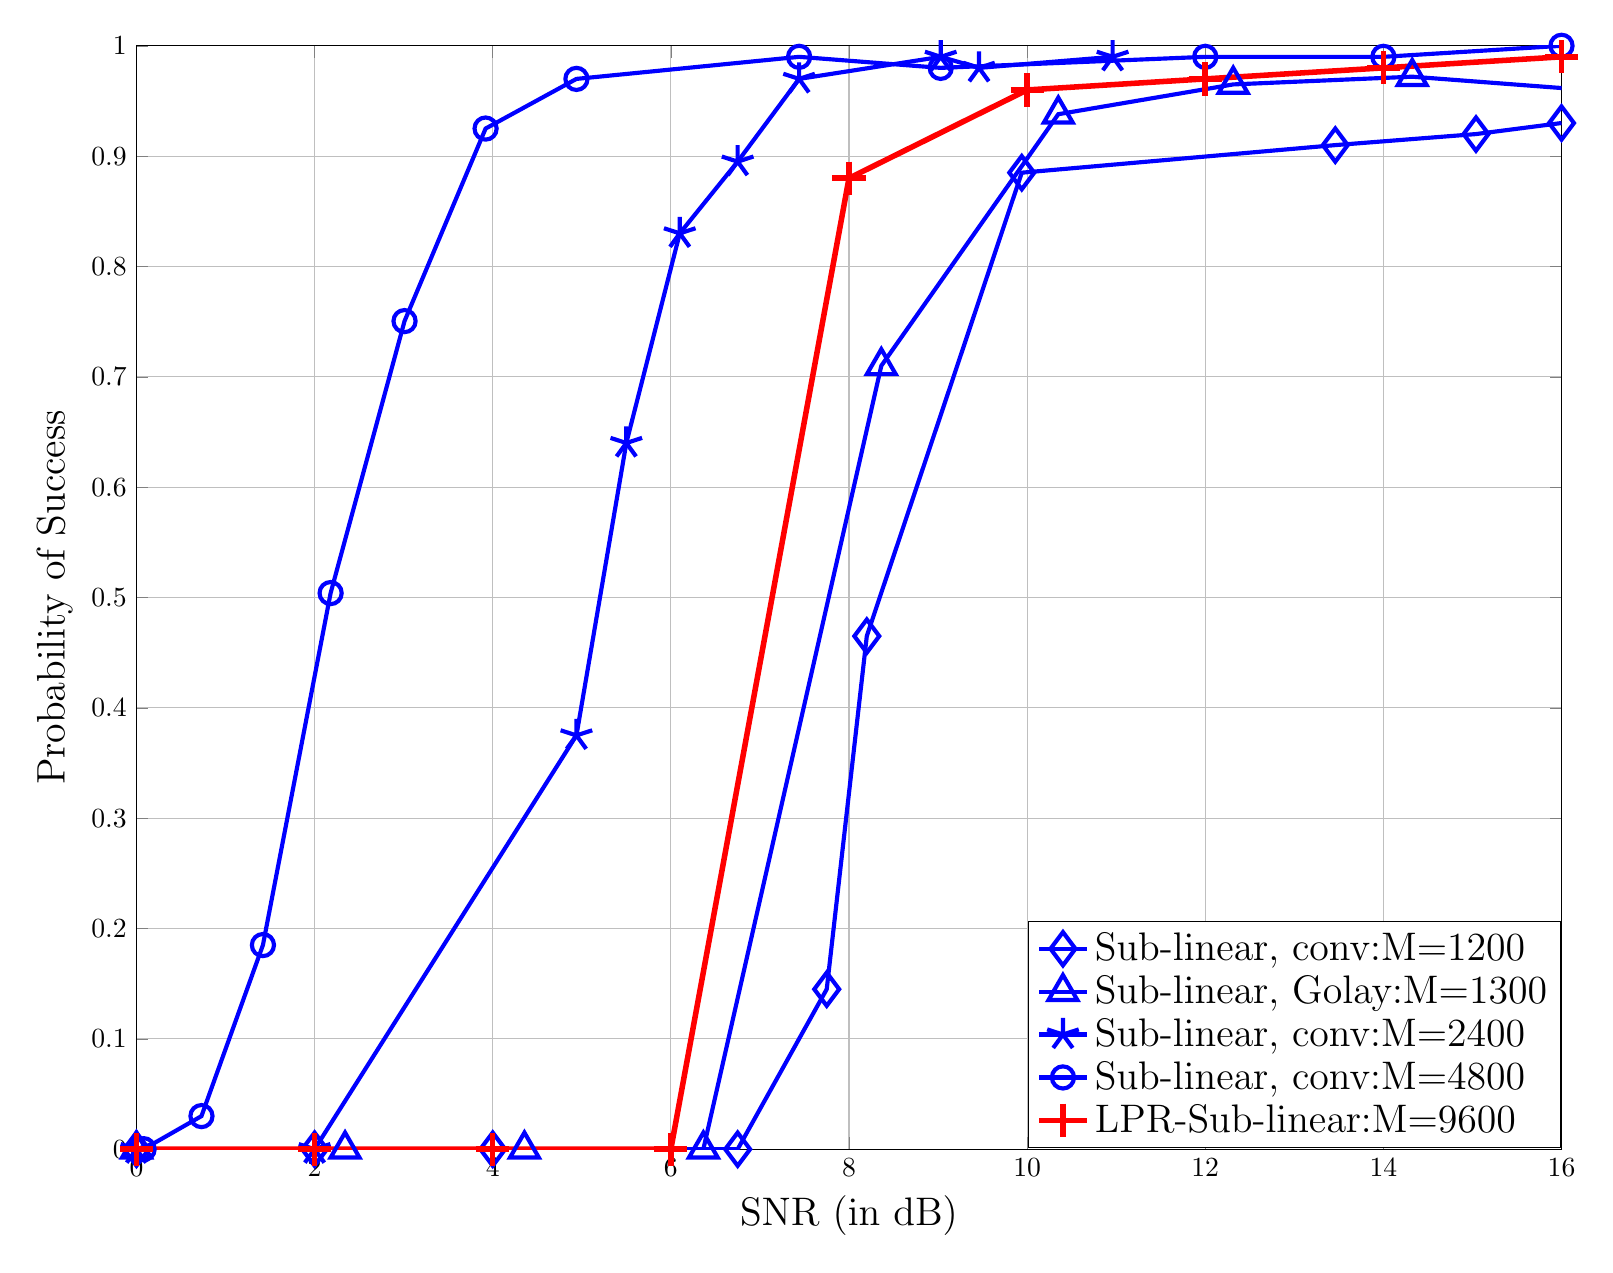
\begin{tikzpicture}

\begin{axis}[%
width=7.12521981627297in,
height=5.51690441819773in,
scale only axis,
xmin=0,
xmax=16,
xmajorgrids,
ymin=0,
ymax=1,
ymajorgrids,
 %xtick = {0,1,2,3,4,5,6,7,8,9,10,11,12,13,14,15,16},
xtick = {0,2,4,6,8,10,12,14,16},
xlabel={\Large{SNR (in dB)}},
ylabel={\Large{Probability of Success}},
legend style={at={(1.0,0.0012)},anchor=south east,draw=black,fill=white,legend cell align=left,font=\Large}
]


%\addplot [color=green,solid,line width=1.5pt,mark size=4.0pt,mark=pentagon,mark options={solid}]
%  table[row sep=crcr]{16	0.95\\
%15.05	0.92\\
%12.12	0.89\\
%9.94	0.875\\
%8.2	0.585\\
%7.81	0.33\\
%7.44	0.115\\
%6.1	0\\
%};
%\addlegendentry{Sub-linear:M=1300};


%Convolutional Code 1/2 rate. No sign row
\addplot [color=blue,solid,line width=1.5pt,mark size=6.0pt,mark=diamond,mark options={solid}]
  table[row sep=crcr]{ 16 0.93\\
  15.04 0.92\\
13.46   0.91\\
9.94   0.8850\\
8.20  0.4650\\
7.75 0.1450\\
6.75 0\\
4 0\\
2  0\\
0	0\\
};
\addlegendentry{Sub-linear, conv:M=1200};

\addplot [color=blue,solid,line width=1.5pt,mark size=6.0pt,mark=triangle,mark options={solid}]
  table[row sep=crcr]{0 0\\
%  2 0\\
%  4 0\\
%  6.1 0.1\\
%  8.01 0.82\\
%  10.043  0.96\\
%  12.0057 0.964\\
%  14 0.97  0.97\\
2.342 0\\
4.356 0\\
6.365 0\\
8.363    0.71\\
10.35    0.938\\
12.314 0.965\\
14.324  0.972\\
 16.28 0.96\\
};
\addlegendentry{Sub-linear, Golay:M=1300};

\addplot [color=blue,solid,line width=1.5pt,mark size=6.0pt,mark=star,mark options={solid}]
  table[row sep=crcr]{0 0\\
  2 0\\
  4.94 0.375\\
  5.50 0.64\\
  6.10 0.83\\
  6.75 0.895\\
  7.44 0.97\\
9.03  0.99\\
  9.46 0.98\\
  10.96 0.99
  13.46 0.985\\
};
\addlegendentry{Sub-linear, conv:M=2400};

\addplot [color=blue,solid,line width=1.5pt,mark size=4.0pt,mark=o,mark options={solid}]
  table[row sep=crcr]{ 16 1\\
  14 0.99\\
  12 0.99\\
  9.03 0.98\\
7.44 0.99
  6.10  0.97\\
  4.94  0.97\\
  3.92  0.925\\
  3.01  0.7505 \\
  2.18  0.504\\
  1.42 0.185\\
  0.73 0.03\\
  0.08 0\\
};
\addlegendentry{Sub-linear, conv:M=4800};

\addplot [color=red,line width=2.0pt,mark size=6.0pt,mark=+,mark options={solid}]
  table[row sep=crcr]{0	0\\
2	0\\
4	0\\
6	0\\
8	0.88\\
10	0.96\\
12	0.97\\
14	0.98\\
16	0.99\\
};
\addlegendentry{LPR-Sub-linear:M=9600};

%\addplot [color=red,dashed,line width=1.5pt,mark size=6.0pt,mark=square,mark options={solid}]
%  table[row sep=crcr]{0	0\\
%2	0\\
%4	0\\
%6	0.005\\
%8	0.08\\
%10	0.215\\
%12	0.43\\
%14	0.58\\
%16	0.65\\
%};
%\addlegendentry{LPR-Near-linear:M=1200};
%
%\addplot [color=red,dashed,line width=1.5pt,mark size=6.0pt,mark=triangle,mark options={solid}]
%  table[row sep=crcr]{0	0\\
%2	0.04\\
%4	0.78\\
%6	0.95\\
%8	0.97\\
%10	1\\
%12	1\\
%14	1\\
%16	1\\
%};
%\addlegendentry{LPR-Near-linear:M=2400};


%\addplot [color=blue,solid,line width=1.5pt,mark size=6.0pt,mark=otimes,mark options={solid}]
%  table[row sep=crcr]{0	0\\
%2.18      0     \\
%3.01 0.0700 \\
%3.92  0.4200 \\
%4.94  0.7400 \\
%6.10  0.9450 \\
%7.44  0.9900 \\
%9       0.999   \\
%12     1.00    \\
%};
%\addlegendentry{BCH-Near-linear:M=2400};


\end{axis}
\end{tikzpicture}%
\end{centering}
}
\caption{Probability of Success for our construction (blue curves) with \emph{BinaryNoisy} scheme using convolutional codes(conv) and Golay code with sub-linear time decoding complexity of $O(K\log \frac{N}{K})$.% and BCH codes with near-linear(red) complexity.  
 And we compare the performance with that of \emph{BinaryNoisy} scheme by Li, Pawar and Ramachandran (LPR) (red curve) \cite{li2015subdraft} with sub-linear decoding complexity of $O\left( K \log N\right)$.} %and \emph{F scheme with near-linear complexity of $O\left(N\log N\right)$. }	

\label{Fig:Sims}	
\end{figure}

\section{Conclusion}
In this chapter we considered the support recovery problem in compressed sensing and proposed a sensing matrix construction based on left-and-right regular sparse-graph ensemble. It was shown that the proposed construction, using an order optimal measurement complexity of $\mc{O}(K\log\frac{N}{K})$, recovers the support of the sparse signal with asymptotically vanishing error probability in optimal sub-linear time complexity of $\mc{O}(K\log\frac{N}{K})$.
%\section{Extensions} % For the group testing problem addressed in \cite{lee2015saffron} also, it appears we can replace the ensemble used by Lee, Pedarsani and Ramchandran by the regular-regular ensemble and obtain a sharper result, i.e., $O(K \log (N/K))$ measurements for the case of $K = N^\delta$, where $\delta < 2/3$.
%%
%%When the right regular ensemble is considered, then the probability of error at each measurement node will be $O\left(\frac{K^2}{N^2}\right)$ and there are $K$ stages in the peeling process. Thus, for the overall error probability to decay with $K$, we require that
%%\[
%%\frac{K^3}{N^2} < 1 \Rightarrow \frac{N^{3\delta}}{N^2} < 1 \Rightarrow \delta < \frac{2}{3}.
%%\]
%%
%%The main idea in the proof is to look at the reduced subgraph induced only by the defective items and when $N/K \rightarrow \infty$, this graph will be a graph from the left regular, right Poisson ensemble considered in \cite{lee2015saffron}.
%
%For the group testing problem addressed in \cite{lee2015saffron} also, it appears we can replace the ensemble used by Lee, Pedarsani and Ramchandran by the regular-regular ensemble and obtain a sharper result, i.e., $O(K \log (N/K))$ measurements for the case of $K = N^\delta$.
%
%We use a left and right regular ensemble for the LDPC code and we use a measurement matrix with $2 \beta \log_2(N/K)$ rows and $N/K$ columns. When the right regular ensemble is considered, then the probability of error at each measurement node will be $O\left(\frac{K^{\beta-1}}{N^{\beta-1}}\right)$ and there are $K$ stages in the peeling process. Thus, for the overall error probability to decay with $K$ according to $O\left(\frac{K^{\beta}}{N^{\beta-1}}\right) = O\left(N^{\delta \beta - \beta + 1}\right)$. If we want this probability of error to be $O(N^{-\delta})$, then we can set $\beta = \frac{1+\delta}{1-\delta}$ to satisfy this. Then, the total number of measurements will be $2 (1+\delta) K \log_2 N$. This is strictly an improvement over $6 K \log_2 N$ measurements used in \cite{lee2015saffron}.
%
%The main idea in the proof is to look at the reduced subgraph induced only by the defective items and when $N/K \rightarrow \infty$, this graph will be a graph from the left regular, right Poisson ensemble considered in \cite{lee2015saffron}.